%%%%%%%%%%%%%%%%%%%%%%%%%%%%%%%%%%%%%%%%%
% Programming/Coding Assignment
% LaTeX Template
%
% This template has been downloaded from:
% http://www.latextemplates.com
%
% Original author:
% Ted Pavlic (http://www.tedpavlic.com)
%
% Note:
% The \lipsum[#] commands throughout this template generate dummy text
% to fill the template out. These commands should all be removed when 
% writing assignment content.
%
% This template uses a Perl script as an example snippet of code, most other
% languages are also usable. Configure them in the "CODE INCLUSION 
% CONFIGURATION" section.
%
%%%%%%%%%%%%%%%%%%%%%%%%%%%%%%%%%%%%%%%%%

%----------------------------------------------------------------------------------------
%	PACKAGES AND OTHER DOCUMENT CONFIGURATIONS
%----------------------------------------------------------------------------------------

\documentclass[a4paper]{article}

\usepackage{fancyhdr} % Required for custom headers
\usepackage{lastpage} % Required to determine the last page for the footer
\usepackage{extramarks} % Required for headers and footers
\usepackage[usenames,dvipsnames]{color} % Required for custom colors
\usepackage{graphicx} % Required to insert images
\usepackage{listings} % Required for insertion of code
\renewcommand*{\lstlistingname}{代码} % change "Listing <ref> to 代码 <ref>
\usepackage{courier} % Required for the courier font
\usepackage{lipsum} % Used for inserting dummy 'Lorem ipsum' text into the template

\usepackage[UTF8]{ctex} % Required for Chinese character
\usepackage{tocloft} % Required for beautiful toc
\usepackage[hidelinks]{hyperref} % Required for clickable toc
\hypersetup{
    colorlinks,
    citecolor=black,
    filecolor=black,
    linkcolor=black,
    urlcolor=black
}
\usepackage[title]{appendix} % Required for appendix

% Margins
\topmargin=-0.45in
\evensidemargin=0in
\oddsidemargin=0in
\textwidth=6.5in
\textheight=9.0in
\headsep=0.25in

\linespread{1.1} % Line spacing

% Set up the header and footer
\pagestyle{fancy}
\lhead{\hmwkAuthorName} % Top left header
\chead{\hmwkClass\ (\hmwkClassInstructor\ \hmwkClassTime): \hmwkTitle} % Top center head
\rhead{\firstxmark} % Top right header
\lfoot{\lastxmark} % Bottom left footer
\cfoot{} % Bottom center footer
\rfoot{Page\ \thepage\ of\ \protect\pageref{LastPage}} % Bottom right footer
\renewcommand\headrulewidth{0.4pt} % Size of the header rule
\renewcommand\footrulewidth{0.4pt} % Size of the footer rule

\setlength\parindent{0pt} % Removes all indentation from paragraphs

%----------------------------------------------------------------------------------------
%	CODE INCLUSION CONFIGURATION
%----------------------------------------------------------------------------------------

\definecolor{MyDarkGreen}{rgb}{0.0,0.4,0.0} % This is the color used for comments
\lstloadlanguages{Perl} % Load Perl syntax for listings, for a list of other languages supported see: ftp://ftp.tex.ac.uk/tex-archive/macros/latex/contrib/listings/listings.pdf
\lstset{language=Perl, % Use Perl in this example
        frame=single, % Single frame around code
        basicstyle=\small\ttfamily, % Use small true type font
        keywordstyle=[1]\color{Blue}\bf, % Perl functions bold and blue
        keywordstyle=[2]\color{Purple}, % Perl function arguments purple
        keywordstyle=[3]\color{Blue}\underbar, % Custom functions underlined and blue
        identifierstyle=, % Nothing special about identifiers                                         
        commentstyle=\usefont{T1}{pcr}{m}{sl}\color{MyDarkGreen}\small, % Comments small dark green courier font
        stringstyle=\color{Purple}, % Strings are purple
        showstringspaces=false, % Don't put marks in string spaces
        tabsize=5, % 5 spaces per tab
        %
        % Put standard Perl functions not included in the default language here
        morekeywords={rand},
        %
        % Put Perl function parameters here
        morekeywords=[2]{on, off, interp},
        %
        % Put user defined functions here
        morekeywords=[3]{test},
       	%
        morecomment=[l][\color{Blue}]{...}, % Line continuation (...) like blue comment
        numbers=left, % Line numbers on left
        firstnumber=1, % Line numbers start with line 1
        numberstyle=\tiny\color{Blue}, % Line numbers are blue and small
        stepnumber=2, % Line numbers go in steps of 5,
        firstnumber=1
}

% Creates a new command to include a perl script, the first parameter is the filename of the script (without .pl), the second parameter is the caption

\newcommand{\shfilescript}[3]{
\begin{itemize}
\item[]\lstinputlisting[caption=#2, label=lst:#1, language=sh]{#3}
\end{itemize}
}
\newcommand{\shscript}[3]{
\begin{itemize}
\item[]\begin{lstlisting}[label=lst:#1, caption=#2] #3 \end{lstlisting}
\end{itemize}
}

%----------------------------------------------------------------------------------------
%	DOCUMENT STRUCTURE COMMANDS
%	Skip this unless you know what you're doing
%----------------------------------------------------------------------------------------

% Header and footer for when a page split occurs within a problem environment
\newcommand{\enterProblemHeader}[1]{
\nobreak\extramarks{#1}{#1 见下页\ldots}\nobreak{} 
\nobreak\extramarks{接上页}{#1 见下页\ldots}\nobreak{}
}

% Header and footer for when a page split occurs between problem environments
\newcommand{\exitProblemHeader}[1]{
\nobreak\extramarks{接上页}{#1 见下页\ldots}\nobreak{}
\nobreak\extramarks{#1}{}\nobreak{}
}
% TODO:code here enable the number before section, but it disable the numbering of problems
%\setcounter{secnumdepth}{0} % Removes default section numbers
\newcounter{homeworkProblemCounter} % Creates a counter to keep track of the number of problems

\newcommand{\homeworkProblemName}{}

\newenvironment{homeworkProblem}[1][Problem \arabic{homeworkProblemCounter}]{ % Makes a new environment called homeworkProblem which takes 1 argument (custom name) but the default is "Problem #"
\stepcounter{homeworkProblemCounter} % Increase counter for number of problems
\renewcommand{\homeworkProblemName}{#1} % Assign \homeworkProblemName the name of the problem
\section{\homeworkProblemName} % Make a section in the document with the custom problem count
\enterProblemHeader{\homeworkProblemName} % Header and footer within the environment
}{
\exitProblemHeader{\homeworkProblemName} % Header and footer after the environment
}

\newcommand{\problemAnswer}[1]{ % Defines the problem answer command with the content as the only argument
\noindent\framebox[\columnwidth][c]{\begin{minipage}{0.98\columnwidth}#1\end{minipage}} % Makes the box around the problem answer and puts the content inside
}

\newcommand{\homeworkSectionName}{}
\newenvironment{homeworkSection}[1]{ % New environment for sections within homework problems, takes 1 argument - the name of the section
\renewcommand{\homeworkSectionName}{#1} % Assign \homeworkSectionName to the name of the section from the environment argument
\subsection{\homeworkSectionName} % Make a subsection with the custom name of the subsection
\enterProblemHeader{\homeworkProblemName\ [\homeworkSectionName]} % Header and footer within the environment
}{
\enterProblemHeader{\homeworkProblemName} % Header and footer after the environment
}


\newcommand{\codev}[1]{\textsf{#1}}
%----------------------------------------------------------------------------------------
%	NAME AND CLASS SECTION
%----------------------------------------------------------------------------------------

\newcommand{\hmwkTitle}{操作系统原理实验\ \#2} % Assignment title
\newcommand{\hmwkDueDate}{Monday,\ March\ 19,\ 2018} % Due date
\newcommand{\hmwkClass}{16级计科\ 7班} % Course/class
\newcommand{\hmwkClassTime}{周一9-10节} % Class/lecture time
\newcommand{\hmwkClassInstructor}{凌应标} % Teacher/lecturer
\newcommand{\hmwkAuthorName}{颜彬} % Your name
\newcommand{\hmwkAuthorId}{16337269} % Your id 

%----------------------------------------------------------------------------------------
%	TITLE PAGE
%----------------------------------------------------------------------------------------

\usepackage{titling}

\title{
\vspace{2in}
\textmd{\textbf{\hmwkClass:\ \hmwkTitle}}\\
\normalsize\vspace{0.1in}\small{Due\ on\ \hmwkDueDate}\\
\vspace{0.1in}\large{\textit{\hmwkClassInstructor\ \hmwkClassTime}}
\vspace{3in}
}

\author{\textbf{\LARGE{\hmwkAuthorName}} \\ \\ \textbf{\LARGE{\hmwkAuthorId}}}
\date{} % Insert date here if you want it to appear below your name
%----------------------------------------------------------------------------------------

\begin{document}
% \begin{titlingpage} % This is for ignore page number in first page. package titling

\maketitle

%----------------------------------------------------------------------------------------
%	TABLE OF CONTENTS
%----------------------------------------------------------------------------------------

\setcounter{tocdepth}{2} % Uncomment this line if you don't want subsections listed in the ToC


\renewcommand{\cftsecleader}{\cftdotfill{\cftdotsep}} % used for dots between <section> and <page>
\renewcommand{\contentsname}{Content} % force the word to be "content
\newpage
\tableofcontents
\addtocontents{toc}{~\hfill\textbf{Page}\par}
\newpage

% below are document body


% To have just one problem per page, simply put a \clearpage after each problem
\section{实验目的}
设计和完善更多的有输出的用户程序。加深对 16位x86汇编的理解。加深对汇编程序中``寻址''的理解,
例如\codev{jmp near}和\codev{jmp far}的区别,和\codev{org}指令的理解。\\

理解bios中断,掌握基础的bios中断的运用,特别是键盘输入中断,字符串输出中断和扇区载入中断。修改并完成控制程序,使其识别
并响应键盘按下事件。\\

理解程序在磁盘和内存中存储方式的不同点。掌握将用户程序载入内存的操作。\\

\section{实验要求}
    \subsection{拓展用户程序}
    设计四个有输出的用户可执行程序,分别在屏幕 1/4 区域动态输出字符,如
    将用字符`A'从屏幕左边某行位置 45 度角下斜射出,保持一个可观察的适当
    速度直线运动,碰到屏幕相应 1/4 区域的边后产生反射,改变方向运动,如
    此类推,不断运动;在此基础上,增加你的个性扩展,如同时控制两个运动
    的轨迹,或炫酷动态变色,个性画面,如此等等,自由不限。还要在屏幕某
    个区域特别的方式显示你的学号姓名等个人信息。
    \subsection{组织存储方式}
    自行组织映像盘的空间,以存放四个用户可执行程序。自行组织内存的空间,以排列控制程序和用户程序等。
    \subsection{响应按键事件}
    修改参考原型代码,允许键盘输入,用于指定运行这四个有输出的用户可执
    行程序之一,要确保系统执行代码不超过 512 字节,以便放在引导扇区
\section{实验方案}
    \subsection{基础原理}
    \subsubsection{NASM宏} 
    NASM具有极其强大的宏功能。NASM宏允许程序在编译时成文本替换、代码生成、表达式运算、引入其他文件代码等强大的工作。\\
    
    本实验要求产生四个及以上的用户程序。本项目利用宏的灵活性,通过调整编译指令,在简单修改源代码的基础上,产生了6个
    用户程序。该6个用户程序分别在屏幕的左上角、上方、右上角、左下角、下方、右下角运动。代码实现如,编译方法见%TODO:finish here
    \subsubsection{独立的全局函数空间} \label{subsec:globalFunc}
    为了增加代码的可拓展性和可组织性,本项目特地增加了``全局函数空间''。即在内存0xA100至0xA300的空间范围内,放置
    本项目常用的函数的实现,如清屏和打印字符串等。0xA100地址起始处的若干字节将保留用作索引信息。其他程序只需要检查
    0xA100之后的若干字节,即可知道目标函数的物理地址,并采用\codev{call [reg]}的方式跳转并执行。具体实现方法xx节的见代码%FIXME: ref
    \subsubsection{组织存储方式}
    真正的磁盘由若干个盘片堆叠而成。每个盘片都有两个磁头,故经常用磁头从上到下的
    编号来代指盘面的编号。每个磁头可以共同步进或步退,在磁盘高速运转时,磁头的每个运行轨迹对应一个磁道。
    将磁道继续细分,每个磁道可分为若干个扇区,通常分为63个,从1编号至63.每个扇区512字节。\\
    
    从实验一可知,第一个扇区为引导扇区,在裸机开机时会被自动加载入内存并尝试引导。本项目还有额外的6个用户程序和1个独立的全局函数程序(见
    \ref{subsec:globalFunc})。在
    本实现中,全局函数程序将占据虚拟软盘的第二个扇区。
    其余的每个用户程序将单独占据一个扇区,并从第三个扇区开始,依次排列。即将第\codev{i}个用户程序放置在虚拟软盘的第
    \codev{i + 2}个扇区内。他们在内存中的存放方式见。。节代码。。。%FIXME: ref
    \\
    
    \subsubsection{bios中断}
    bios提供了若干基本的中断供程序调用。其中包括字符(串)输出中断,键盘中断和扇区载入中断等。在程序中,只需要将正确的参数
    置于相应的寄存器中,并执行\codev{int <num>}即可直接调用相应的中断。本程序使用的中断见附录中断表%FIXME: ref
    \\
    \subsubsection{程序寻址}
    由于本项目除了引导程序外,还具有数个其他程序,代码段间的跳转和数据的寻址显得尤其重要。在x86实模式下,寻址采用的方式是
    $$ addr = segment \times 16 + offset $$
    其中,在十六进制下又等价为 $$addr = segment \ll 1 + offset$$.
    \\
    
    值得注意的是,\codev{jmp near}和\codev{jmp far}将具有不同的行为。前者不会改变段寄存器,而后者会将段寄存器修改为目标位置的段基地址。
    在本项目中,所有跳转都采用\codev{jmp near}的方式。 \\
    
    在本项目中,\codev{org}的使用尤其关键。对于它的使用见..节代码。。%FIXME: ref
    %TODO: 在这里解释org!!!
    \subsubsection{键盘响应} \label{subsec:kbhandler}
    对按键的响应主要通过16H系统中断完成。本项目主要使用16号中断的00H功能和01H功能。\\ 
    
    01H功能会检查键盘缓冲区的内容。若缓冲区为空,ax将保持不变。若缓冲区中按键缓冲,
    则ah会被修改,而al将存储按下键的ascii码。\\
    
    00H的功能和01H十分相似。两者最大的不同在于对缓冲区的处理。01H功能调用在检查缓冲区后,会保留缓冲区不变。
    这意味着,若缓冲区不为空,连续的多次使用01H号功能将得到相同的返回内容。而00H则不同,它在检查缓冲区后,若缓冲区
    不为空,则会将缓冲区的头部取出(相当于队列的出队操作);若缓冲区为空,程序会被阻塞直到键盘被按下。\\ 

    关于按键响应的详细使用,见\ref{subsec:kbhandler}节。

    \subsubsection{实验环境}
        \begin{itemize} \item 操作系统 \\ 
            本实验在Linux下完成。采用Ubuntu 16.04
            \item 虚拟机\\
            bochs.它是一款开源且跨平台的 IA-32 模拟器。
        \end{itemize}
    \subsubsection{相关工具、指令}
        \begin{itemize}
            \item 汇编器\\ 
            NASM. NASM是一个轻量级的、模块化的 80x86 和 x86-64 汇编器。它的语法与
            Intel 原语法十分相似,但更加简洁和易读。它对宏有十分强大的支持。
            \item 镜像文件产生工具\\ 
            bximage. 该命令允许生成指定大小的软件镜像。
            \item 二进制写入命令\\ 
            dd. dd 允许指定源文件和目标文件,将源文件的二进制比特写入目标文件中的指定位置。
            \item 二进制文件查看命令\\ 
            xxd. xxd 允许将二进制文件中的内容按地址顺序依次输出,可读性强
        \end{itemize}
    \subsection{程序流程}\label{subsec:programProcedure}
    图\ref{fig:overview}展示了程序整体间的关联方式。控制程序在获得处理器控制权后,立即将全局函数模块
    载入内存中。在清屏和输出相关的提示信息后,等待键盘按下。\\
    
    每当键盘被按下,控制程序会判断按下的是哪个键,并把相应的用户程序载入内存中,随后运行用户程序。在用户程序的
    运行期间,若用户程序检测到键盘按下,它会先把控制权返回给控制程序,由控制程序统一处理。而控制程序使用到的
    所有函数,由全局函数模块统一管理。\\
    
    图\ref{fig:program}展示了用户程序的流程图。该流程与实验一的流程图十分相似。不同之处在于,每个循环内,
    用户程序需要检查键盘是否被按下。若键盘被按下,需要将控制权返回给控制程序。

    
    \begin{figure}
        \begin{center}
        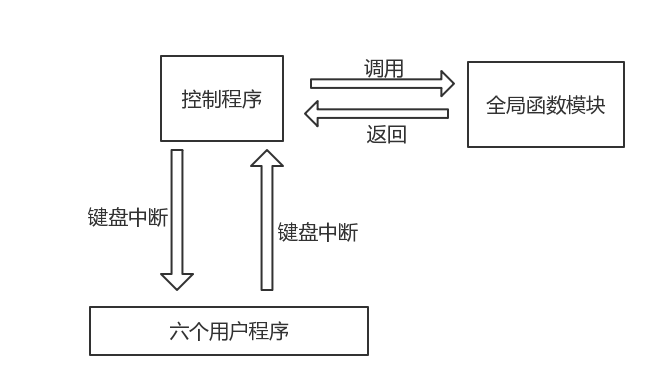
\includegraphics[scale=0.4]{assets/overview.png}
        \caption{程序间关联方式\label{fig:overview}}
        \end{center} 
    \end{figure} 
    
    
    \begin{figure}
        \begin{center}
        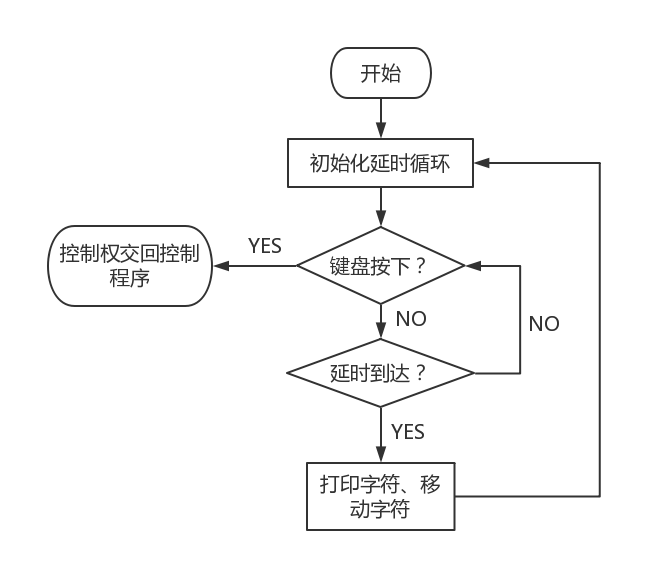
\includegraphics[scale=0.4]{assets/program.png}
        \caption{用户程序流程图\label{fig:program}} 
        \end{center} 
    \end{figure} 
    
    
    \subsection{程序模块及相关说明}\label{subsec:modelIntroduction}
    \subsubsection{NASM宏} \label{subsec:NASMmacro}
    为了产生6个互不相同的用户程序,本代码充分利用了NASM的宏特性。如代码\ref{lst:userMacro}所示。\\
    
    首先,若编译时带有\codev{DEBUG}选项,则会使delay被定义为1000,否则delay为50000。以这个方式定义delay变量
    是由于bochs虚拟机的性能较差,
    若delay的值较大会导致程序运行速度过低,查错变得更难。但其他虚拟机的运行速度比bochs
    快,需要更大的delay才能让程序的动画肉眼可见。故这里根据是否定义了\codev{DEBUG}宏而给出了两种不同的延时。
    通过简单地修改编译指令,可以使得编译后的程序适应多种机型(和虚拟机)。\\
    
    随后,根据程序的六种不同的位置(如左上、右上、左下等),定义了6个不同的宏。通过在编译时指出不同的宏,
    程序将被编译出6种不同的版本。如此即可在几乎不修改代码的前提下产生众多相似程序。
    这六个不同的宏中,每个宏各自定义了符号的起始坐标\codev{x}和\codev{y},上下左右的四个边界
    的坐标\codev{[(Down)|(Up)|(Left)|(Right)]SideBound},符号的初始运行方向和程序的偏移地址等。\\
    

    程序的编译方法对程序的产生具有重大影响。编译命令见%FIXME: ref
    。\\
    
    宏中\codev{org}指令的解释见%FIXME:ref
    
    \begin{figure}
    \begin{itemize}
    \item[] \begin{lstlisting}[language={[x86masm]Assembler}, label=lst:userMacro, caption=用户程序中的部分宏代码]
; in file stone.asm 

%ifdef DEBUG
    delay equ 1000
%else
    delay equ 50000
%endif

%ifdef UL
    mycode equ 'q'
    DownSideBoundary equ 12
    UpSideBoundary equ 4
    LeftSideBoundary equ 1
    RightSideBoundary equ 23
    _x equ 1
    _y equ 10
    org 0A300H
    DIRECTION equ Up_Lt
%elifdef UP
    ; ...
    ; ...
%endif
    \end{lstlisting}
    \end{itemize}
    \end{figure}
   

    \subsubsection{键盘响应}
    对键盘的响应和中断的使用见\ref{subsec:kbhandler}节的介绍。本节主要对程序代码中的相关部分做解释。\\

    代码\ref{lst:userKbPress}介绍了用户程序中的按键响应方法。\\
    
    用户程序的主体部分是一个延时循环。每次循环时,程序都会跳转到test\_key\_press过程.程序首先
    检查是否有键按下,若没有,则跳转到下一次的延时循环。若有,程序再检测按下的键是否合法,若不合法,同样跳转到下一次循环。
    若按键合法,则程序会调用一个函数,并将控制权交给控制程序。在进入函数之前,程序首先会做一些准备工作,例如向寄存器中存入传递
    的参数等。随后,程序将sys\_base的值置入bx中。sys\_base指向一系列常用函数的``地址表''的表头。其中按键响应函数的地址在地址表的偏移量
    0AH处。故\codev{call [bx + 0AH]}指令会直接调用键盘响应函数。 \\
     
    有关全局函数地址表和全局函数的问题,见代码%FIXME: ref
    
    \begin{figure}
    \begin{itemize}
    \item[] \begin{lstlisting}[language={[x86masm]Assembler}, label=lst:userKbPress, caption=用户程序中对键盘按下的响应]
    ; in file stone.asm
    test_key_press:
        xor ax, ax
        mov ah, 1
        int 16H
        cmp ah, 1
        jz loop1.Loop ; if no key is pressed, jump to delay loop

        xor ax, ax
        int 16H
        cmp al, mycode
        jz loop1.Loop ; if pressed key stand for the program itself
                      ; then just ignore it
        ; key pressed

        ; ...
        ; some set-ups
        ; ...

        mov bx, sys_base
        jmp [bx + 0AH] ; jump to a key-press handler
    \end{lstlisting}
    \end{itemize}
    \end{figure}

    \subsubsection{全局函数}
    为了减少控制模块的代码体积,减少各个模块间的耦合度,以及增加可拓展性,本实验将各个程序间共同需要使用的
    函数抽取出来。当需要调用这些共享函数时,只需要查阅0xA100地址起始处的一个表,找到函数入口地址即可。\\ 

    如代码\ref{lst:utility}所示,该代码段首先声明了\codev{org 0A100H},这是因为控制函数会把该其载入到
    内存0xA100处。紧接着代码段声明了若干个单字长的空间,每个空间存储着对应函数的入口地址。例如\codev{\_show\_at\_call}
    (0xA104H处)这一16位空间存储着函数\codev{show\_at\_call}的入口的地址。每个地址空间声明为16位长(dw)而不是其他的
    长度是因为,8位太短,很可能不足以表示部分函数的地址;不声明为32位或以上的原因是,每个段的段长最多为16位,在不改变
    段寄存器的前提下,16位刚刚好足以表示所有段内函数的地址。\\
    
    在该代码段中,\codev{loader\_address}和\codev{loader\_back\_addres}是两个比较特殊的表项。他们分别指向控制
    程序的首地址和控制程序中按键响应函数的首地址。他们的值在控制程序中会被改写,修改为正确的值。\\
    
    使用这些全局函数的方法很简单。由于这些函数会被载入到内存地址0xA100处,故只需先将bx的值赋为0xA100,并采用
    \codev{call near [bx + offset]}即可。
    \begin{figure}
    \begin{itemize}
    \item[] \begin{lstlisting}[language={[x86masm]Assembler}, label=lst:utility, caption=全局函数和其地址表的定义]
; in file Utilities/utility.asm
org 0A100H
loader_address dw 0xF0F0 ; 0xA100H        0xA100H + 0
loader_back_address dw 0xF0F0 ; 0xA102H        0xA100H + 2
_show_at_call dw show_at_call ; 0xA104H        0xA100H + 4
; ... 
; more items here
; ...
show_at_call:
    ; bp point to str address
    ; cx contents the length
    mov ah, 0EH
    push bx
    mov bl, 0
    mov al, '@'
    int 10H
    pop bx
    jmp [loader_back_address]

; ...
; more functions here
; ...
    \end{lstlisting}
    \end{itemize}
    \end{figure}

    \subsubsection{扇区载入}
    控制程序需要将其他的程序载入到内存中。在本项目中,控制程序还要尽早将全局函数加载入
    内存,以便控制程序(和用户程序)调用其中的函数。\\
    
    同时,当对应的按键被按下时,控制程序还应载入相应的用户程序到相应的内存地址,并跳转到该
    内存地址以执行用户程序。\\
    
    控制程序的代码见代码\ref{lst:loader}.

    \begin{figure}
    \begin{itemize}
    \item[] \begin{lstlisting}[language={[x86masm]Assembler}, label=lst:loader, caption=控制程序中的扇区载入部分]
; in file loader.asm

; ...
; after a key has pressed
; ...
;   mov cl, 3
;   mov bx, 0xA300
    call load
    jmp bx


    load:
    ; cl the nth sector to load
    ; bx the base address to put the code
.body:
    mov ax, 0
    mov es, ax ; which segment to load
    mov ah, 2 ; function number
    mov al, 1 ; load one sector
    mov dx, 0 ; dl = 0 for floppy disk, dh = 0 for 0 head
    mov ch, 0 
    int 13H ; TODO: unkown bugs
    ret 
    \end{lstlisting}
    \end{itemize}
    \end{figure}

\section{实验过程}
    \subsection{编译方法}
    如代码\ref{lst:shbuild}所示,编译本个项目的方法已经封装成脚本build.sh。该脚本会递归地
    调用Utilities/build.sh和userCodes/build.sh,完成这些组件的编译过程。\\ 

    其中userCodes/build.sh的内容如代码\ref{lst:userCodesBuild}所示。该代码在使用
    nasm六次编译文件时,都给出了-D DEBUG的选项。该选项的介绍见\ref{subsec:NASMmacro}.
    这六个文件,在编译时各给出了UL,UP,UR,DL,DN,DR六个选项,分别代表从左上到右下的六个不同
    方向。在编译完成后。这六份代码中的字符'A'会以不同的位置和角度在各自的区域内反射。\\ 

    其中将二进制代码写入虚拟软盘的代码如\ref{lst:build}所示。\\
    boot.bin作为引导程序和控制程序放在第一个扇区。utility.bin作为全局函数放在第二个扇区。
    其余用户程序依次放在连续的扇区中。sh脚本采用"\$((expr))"的方式计算各个bin文件的放置位置。

    \begin{figure}
    \begin{itemize}
    \item[] \begin{lstlisting}[language=sh, label=lst:shbuild, caption=编译程序代码的方法]
$ sh build.sh
    \end{lstlisting}
    \end{itemize}
    \end{figure}

    \begin{figure}
    \begin{itemize}
        \item[]\lstinputlisting[language=sh, label=lst:userCodesBuild, caption=userCodes/build.sh文件内容]{../userCodes/build.sh}
    \end{itemize}
    \end{figure}


    \begin{figure}
    \begin{itemize}
    \item[] \begin{lstlisting}[language=sh, label=lst:build, caption=caption]
dd if=loader.bin of=boot.img conv=notrunc
dd if=Utilities/utility.bin of=boot.img conv=notrunc oflag=seek_bytes seek="$((512*1))"
dd if=userCodes/ul.bin of=boot.img conv=notrunc oflag=seek_bytes seek="$((512*2))"
dd if=userCodes/up.bin of=boot.img conv=notrunc oflag=seek_bytes seek="$((512*3))"
// ...
// ...
dd if=userCodes/dr.bin of=boot.img conv=notrunc oflag=seek_bytes seek="$((512*7))"

    \subsection{运行方法}
    本项目的运行方法与项目一的运行方法一致。\\
    
    运行的方法同样被封装成一个脚本,直接运行即可。见附录\ref{sec:utilitycode}的代码\ref{lst:run}.
    其中文件run.sh的内容见附录\ref{sec:utilitycode}的代码\ref{lst:shrun}.此处不再赘述。

    
    \end{lstlisting}
    \end{itemize}
    \end{figure}
\section{实验结果}
    \lipsum[1]
\section{实验总结}
    \subsection{心得体会}
    \lipsum[1]
    \subsection{遇到的BUG}
        \subsubsection{缓冲区溢出}
        \subsubsection{数据范围错误}

\begin{appendices}
\section{参考文献} \label{sec:reference}
\begin{enumerate}
    \item http://www.nasm.us/doc/ \\
    for nasm
    \item https://en.wikibooks.org/wiki/X86\_Assembly \\
    for 32bit x86
  \end{enumerate}
    \section{辅助代码}\label{sec:utilitycode}
    \begin{figure}
    \begin{itemize}
    \item[] \begin{lstlisting}[language=sh, label=lst:run, caption=运行本项目的方法]
$ sh run.sh
    \end{lstlisting}
    \end{itemize}
    \end{figure}
    \begin{figure}
    \begin{itemize}
        \item[]\lstinputlisting[language=sh, label=lst:shrun, caption=run.sh文件内容]{../run.sh}
    \end{itemize}
    \end{figure}
\end{appendices}
\end{document}